%18/09 - Patricia Álvarez
\chapter{Inferencia bayesiana (BI)}
La inferencia bayesiana se basa en la \textbf{probabilidad posterior} de un árbol condicionada por la matriz observada (alineamiento de secuencias): la probabilidad de que el árbol sea correcto dados los datos. La máxima verosimilitud examina modelos cuyos parámetros son constantes, y obtiene la verosimilitud de obtener los datos dados esos parámetros. La inferencia bayesiana también usa la verosimilitud de los datos, pero usando modelos cuyos parámetros son variables aleatorias con distribuciones estadísticas. 

Antes del análisis de los datos, se asigna una distribución inicial a los parámetros del modelo (prior), que combinada con la verosimilitud de los datos permite calcular la probabilidad posterior de dichos parámetros. El teorema de Bayes sirve para calcular esa probabilidad: la probabilidad del árbol dados los datos es la probabilidad de los datos dado el árbol (likelihood) por la probabilidad inicial del árbol (prior) entre la probabilidad de los datos a través de todos los árboles.

$$ Pr(H|D) = \frac{Pr(D|H) * Pr(H)}{Pr(D)}$$

No se puede calcular el denominador de la expresión, que es la probabilidad inicial de un árbol. Sin embargo, sí se puede aproximar la probabilidad posterior usando un procedimiento de muestreo que se acelera mediante simulaciones de Monte Carlo con cadenas de Markov (MCMC). La idea es vagar al azar en el espacio de árboles de manera que se genera una distribución de árboles cuya media es la de la distribución deseada (la probabilidad Bayesiana). Así, la inferencia bayesiana utiliza MCMC como herramienta para explorar todos los árboles posibles. Hace una buena aproximación del paisaje tras el periodo de “burnin”. Como burnin se conocen las primeras búsquedas al estar más alejadas de los árboles más probables (hay un consenso de quitar el primer 20\% de las búsquedas por este efecto). Cuanto más tiempo corre el procedimiento MCMC (más generaciones), mejor es la aproximación. Conviene repetir el proceso empezando desde diferentes puntos (random seeds).

\begin{figure}[htbp]
\centering
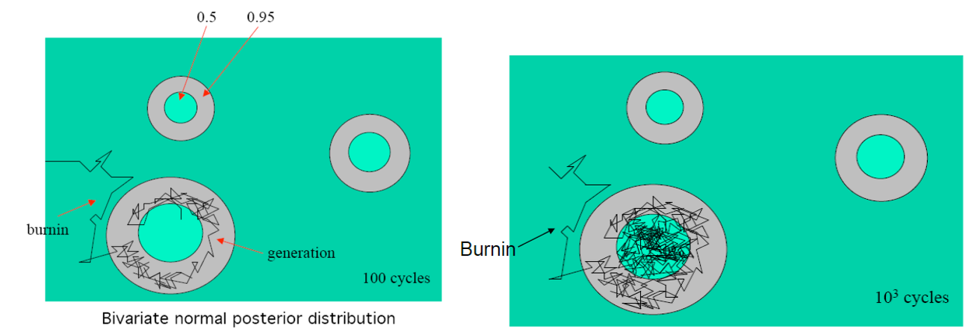
\includegraphics[width=0.5\linewidth]{figs/mcmc.png}
\caption{Aproximación del paisaje por MCMC tras 100 (izquierda) y 10000 (derecha) generaciones.}
\end{figure}

Se realizan dos búsquedas. Las cadenas frías contienen colinas altas y valles profundos. Las cadenas calientes son paisajes en los que la travesía entre colinas es más fácil. En un paisaje frío (típico de las distribuciones de parámetros) es fácil atascarse en óptimos locales. Por ello, se utilizan técnicas de mezclado para resolver el problema de los óptimos locales: se busca que las dos cadenas sean convergentes. Los criterios de convergencia son: 
\begin{itemize}
\item Las distribuciones posteriores de los parámetros del modelo son similares entre cadenas independientes.
\item Las probabilidades posteriores de los clados son similares entre cadenas independientes comenzadas con topologías aleatorias (desviación estándar promedio de las frecuencias divididas).
\end{itemize}

\begin{figure}[htbp]
\centering
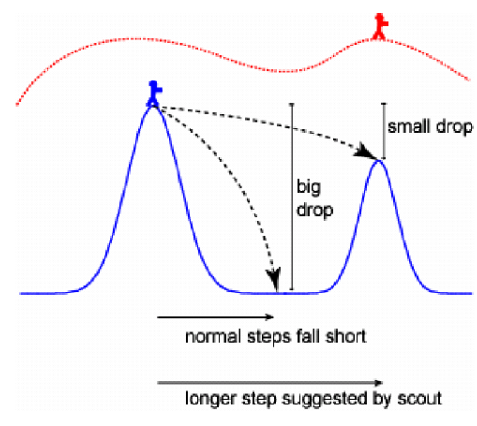
\includegraphics[width=0.5\linewidth]{figs/cadenas-frias-calientes.png}
\caption{Representación gráfica de la búsqueda de cadenas frías (azul) y calientes (rojo).}
\end{figure}

En la práctica, se empieza el procedimiento de MCMC con un árbol aleatorio y un modelo con parámetros aleatorios. En cada generación, y al azar, se propone un nuevo árbol (que se acepta o se rechaza) y un nuevo valor para los parámetros del modelo (que se acepta o se rechaza). Se ejecutan en paralelo una cadena fría y varias calentadas (que orientan a la fría a través del espacio de árboles), mediante un procedimiento MCMCMC. Cada k generaciones, se muestrea los valores de los parámetros de la cadena fría. Tras n generaciones se obtiene una distribución muestral (la cadena fría habrá pasado más tiempo en los mejores lugares del espacio de árboles) y una desviación estándar de las frecuencias divididas.

El método de inferencia Bayesiana calcula una \textbf{probabilidad posterior (BPP)} para cada nodo, que va del 0 al 1. La interpretación estadística es inmediata: es la \textbf{probabilidad de que el clado sea cierto, dado un modelo, unas premisas y unos datos}. Sin embargo, las BPP suelen ser sospechosamente altas (tendencia a la sobreestimación), mucho más que los valores de apoyo de bootstrap. Por ello, se suelen quedar con los valores bayesianos a partir de un 0.9, pero un bootstrap a partir de 70.

\begin{figure}[htbp]
\centering
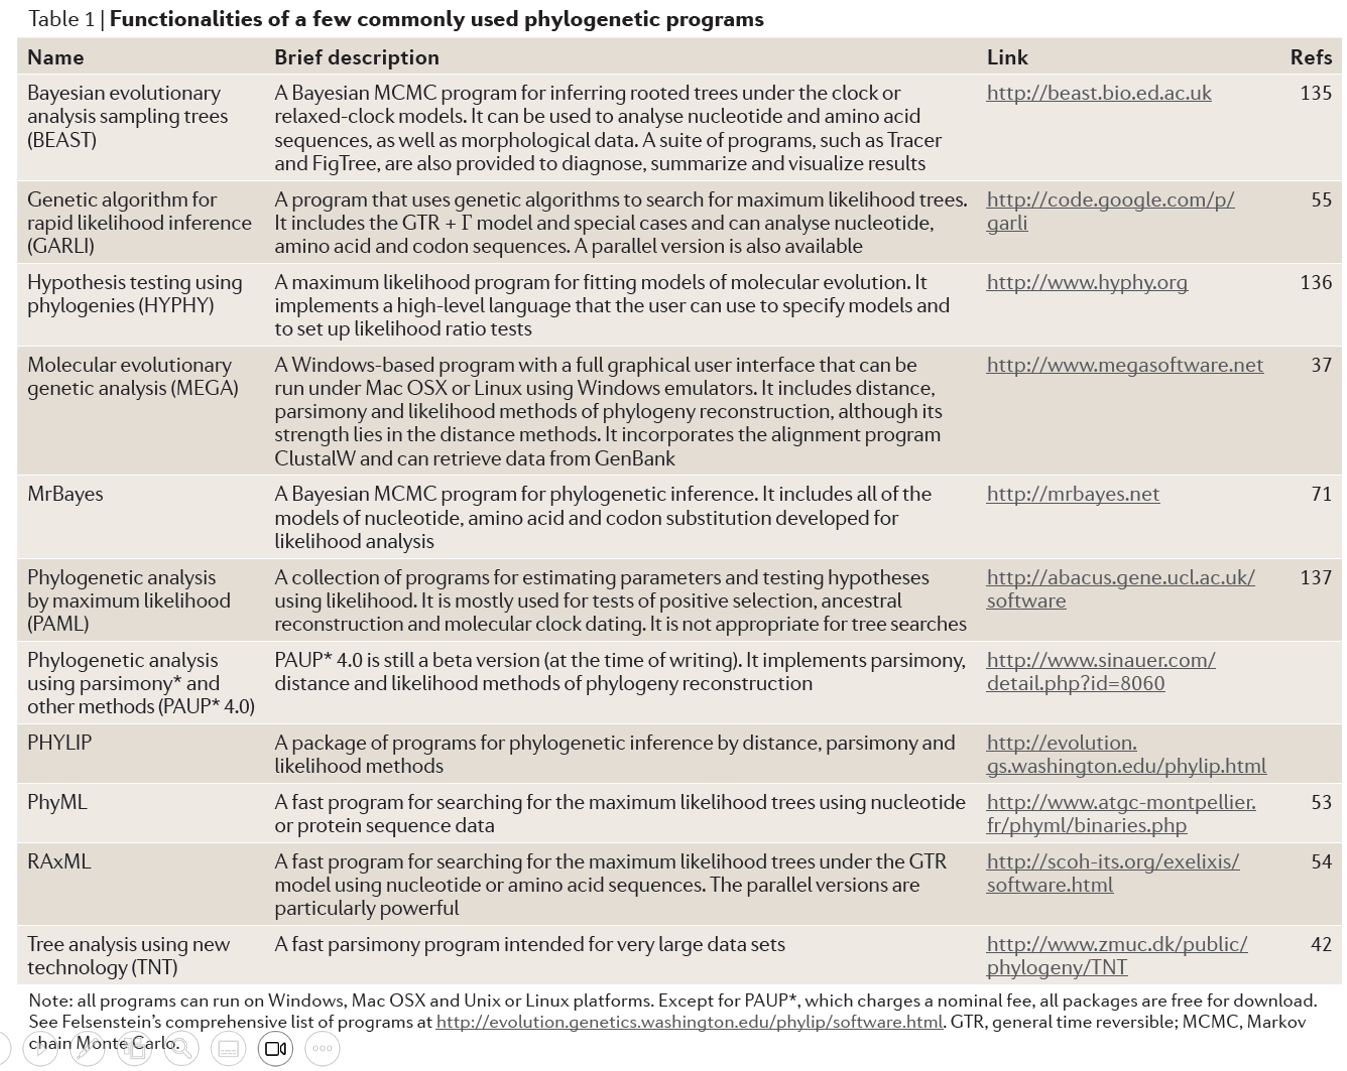
\includegraphics[width=\linewidth]{figs/programas-filogenia.png}
\caption{Lista de los programas más utilizados en filogenia.}
\end{figure}